\documentclass[xcolor={dvipsnames},aspectratio=169,10pt]{beamer}
% utility packages
\usepackage{etoolbox}
\usepackage{multicol}
\usepackage{relsize}
\usepackage{fontawesome}

% better text justifying
\usepackage{microtype}
% justify text inside list environment
% Ref: http://liam0205.me/2017/04/11/justifying-in-beamer-s-lists/
\usepackage{ragged2e}
\makeatletter
\patchcmd{\itemize}{\raggedright}{\justifying}{}{}
\patchcmd{\beamer@enum@}{\raggedright}{\justifying}{}{}
\patchcmd{\@@description}{\raggedright}{\justifying}{}{}
\makeatother

% table of content with numbers and justification
% https://tex.stackexchange.com/questions/188773
\setbeamertemplate{section in toc}{\hspace*{1em}\inserttocsectionnumber.~\inserttocsection\par}
\setbeamertemplate{subsection in toc}{\hspace*{2em}\inserttocsectionnumber.\inserttocsubsectionnumber.~\inserttocsubsection\par}

% math related packages
\usepackage{amsmath}
\usepackage[ruled,vlined]{algorithm2e}
\SetAlCapNameFnt{\scriptsize}
\SetAlCapFnt{\scriptsize}
\SetAlFnt{\scriptsize}

% figure related packages
\usepackage{graphicx}
\usepackage[scale=2]{ccicons}
\usepackage{qrcode}
\usepackage{tikz}
\usepackage{tikzpagenodes}
\usetikzlibrary{positioning}

% table related packages
\usepackage{array}
\usepackage{booktabs}
\usepackage{multirow}
\usepackage{colortbl}
\newcommand{\tabincell}[2]{\begin{tabular}{@{}#1@{}}#2\end{tabular}}

% code highlight
\usepackage{listings}
\usepackage{minted}
\definecolor{mintedbg}{HTML}{E5E9F0}
\setminted{autogobble,bgcolor=mintedbg,fontsize=\small}
\setmintedinline{bgcolor=mintedbg,fontsize=\smaller}
\newminted{bash}{}
\newminted{latex}{}
\newmintinline{bash}{}
\newmintinline{latex}{}
\newcommand{\texdoc}[2]{\href{#2}{\bashinline|texdoc #1|}}

% hyperref setting
\hypersetup{
  unicode,
  psdextra,
  bookmarksnumbered=true,
  bookmarksopen=true,
  bookmarksopenlevel=3,
  bookmarksdepth=4,
  pdfcenterwindow=true,
  pdfstartview={Fit},
  pdfpagemode={FullScreen},
  pdfpagelayout={SinglePage},
}
\usepackage{bookmark}

% beamer theme
\usetheme{metropolis}
\metroset{block=fill,numbering=fraction}

% caption style
\usepackage{subcaption}
\setlength\abovecaptionskip{3pt}
\setbeamerfont{caption}{size=\scriptsize}
\renewcommand{\figurename}{Fig.}
\captionsetup{labelformat=empty,labelsep=none,textfont={bf,it}}

% Ref: https://github.com/gpoore/minted/blob/master/source/minted.dtx
\newenvironment{latexexample}
{\VerbatimEnvironment\begin{VerbatimOut}[gobble=3]{example.out}}{\end{VerbatimOut}%
  \begin{center}
    \begin{minipage}{0.47\linewidth}%
      \inputminted[resetmargins,fontsize=\scriptsize]{latex}{example.out}%
    \end{minipage}%
    \hspace{0.05\linewidth}%
    \begin{minipage}{0.47\linewidth}%
      \begin{framed}
        \setlength{\parindent}{2em}%
        \input{example.out}%
      \end{framed}
    \end{minipage}%
  \end{center}
}

\newenvironment{mathexample}
{\VerbatimEnvironment\begin{VerbatimOut}[gobble=3]{example.out}}{\end{VerbatimOut}%
  \begin{center}
    \begin{minipage}{0.47\linewidth}%
      \inputminted[resetmargins,fontsize=\scriptsize]{latex}{example.out}%
    \end{minipage}%
    \hspace{0.05\linewidth}%
    \begin{minipage}{0.47\linewidth}%
      \begin{framed}
        \[ \input{example.out} \]
      \end{framed}
    \end{minipage}%
  \end{center}
}

\newenvironment{mathexamples}
{\VerbatimEnvironment\begin{VerbatimOut}[gobble=3]{example.out}}{\end{VerbatimOut}%
  \begin{center}
    \begin{minipage}{0.47\linewidth}%
      \inputminted[resetmargins,fontsize=\scriptsize]{latex}{example.out}%
    \end{minipage}%
    \hspace{0.05\linewidth}%
    \begin{minipage}{0.47\linewidth}%
      \begin{framed}
        \directlua{
          local first = true
          for line in io.lines('example.out') do
          if first then
          first = false
          else
          tex.print('\\newline ')
          end
          tex.print('$' .. line .. '$')
          end
        }
      \end{framed}
    \end{minipage}%
  \end{center}
}



%---------------------------------------------------------------------
% Add Paper using {\paper{}. begin{beawer} ... end{beamer} }
%---------------------------------------------------------------------
\newcommand\paper[1]{
	\setbeamertemplate{footline}
	{
		\begin{beamercolorbox}[wd=\textwidth,ht=3mm,dp=03mm,leftskip=0.3cm,rightskip=0.3cm]{black}%
        		\usebeamerfont{page number in head/foot}
			(#1)\mbox{}\hfill\insertframenumber
		\end{beamercolorbox}%
	}
}


\title{air4children: Artificial Intelligence and Robotics for Children}
%\subtitle{...}
\author{
R. Montenegro,
E. Corona,
D. Badillo-P\'erez,
A. Mandujano,
D. Cruz,
{\bf Miguel Xochicale}
}
\date{
Workshop on Child-Robot Interaction \& Child's Fundamental Rights at {\bf \#HRI2021} \\
March 08, 2021
}
\institute{
	\faEnvelope   air4children@gmail.com \\
	\faGithubAlt @air4children \faTwitter @air4children  
		}

\titlegraphic{
  \begin{tikzpicture}[overlay, remember picture]
    \node[%
      above right=0.35cm and -0.2cm of current page footer area.south west,
      anchor=south west,
      inner sep=0pt] {%
      \usebeamerfont{footline}
      \begin{tabular}{lm{.8\textwidth}}
        \href{http://creativecommons.org/licenses/by/4.0/}{\ccby} &
        This slices is licensed under a
	\href{http://creativecommons.org/licenses/by/4.0/}
		{Creative Commons ``Attribution 4.0 International''} license. 
	\par Get source of this slides and see further references 
		from \url{https://github.com/air4children/hri2021}.
      \end{tabular}
    };
    \node[%
      above left=0.35cm and 0cm of current page footer area.south east,
      anchor=south east,
      inner sep=0pt]{\qrcode[height=1.5cm]{https://github.com/air4children/hri2021}};
  \end{tikzpicture}
}

\begin{document}

\maketitle

\begin{frame}{Contents}
    \tableofcontents
\end{frame}

%%%%%%%%%%%%%%%%%%%%%%%%%%%%%%%%%%%%%%%%%%%%
\section{Introduction}

%%%%%%%%%%%%%%%%%%%%%%%%%%%%%%%%%%%%%%%%%%%%%
%\subsection{Subsection}

%%%%%%%%%%%%%%%%%%%%%%%%%%%%%%%%%%%%%%%%%%%%%%%%%%%%%%%%
{
\paper{Lastname N. YEAR in journal of...}
\begin{frame}{The sonographer-probe-patient control system}
      \begin{figure}
        \centering
        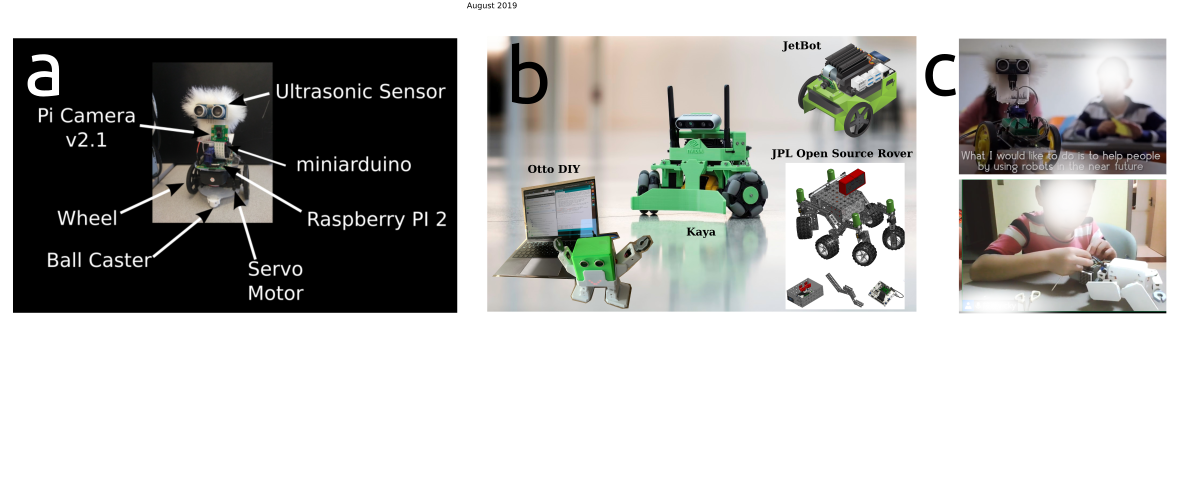
\includegraphics[width=1.0\textwidth]{./figures/air4children/versions/drawing-v02.png}
        %\caption{}
      \end{figure}
\end{frame}
}

%%%%%%%%%%%%%%%%%%%%%%%%%%%%%%%%%%%%%%%%%%%%
\section{AIR4Children}

%%%%%%%%%%%%%%%%%%%%%%%%%%%%%%%%%%%%%%%%%%%%%
\subsection{Prototyping and Piloting Open Source Robots}

%%%%%%%%%%%%%%%%%%%%%%%%%%%%%%%%%%%%%%%%%%%%%%%%%%%%%%%%
{
\paper{Xochicale M. 2014 \it{Libre Robotics (proposal)} }
\begin{frame}{Prototyping Open Source Robots}
      \begin{figure}
        \centering
        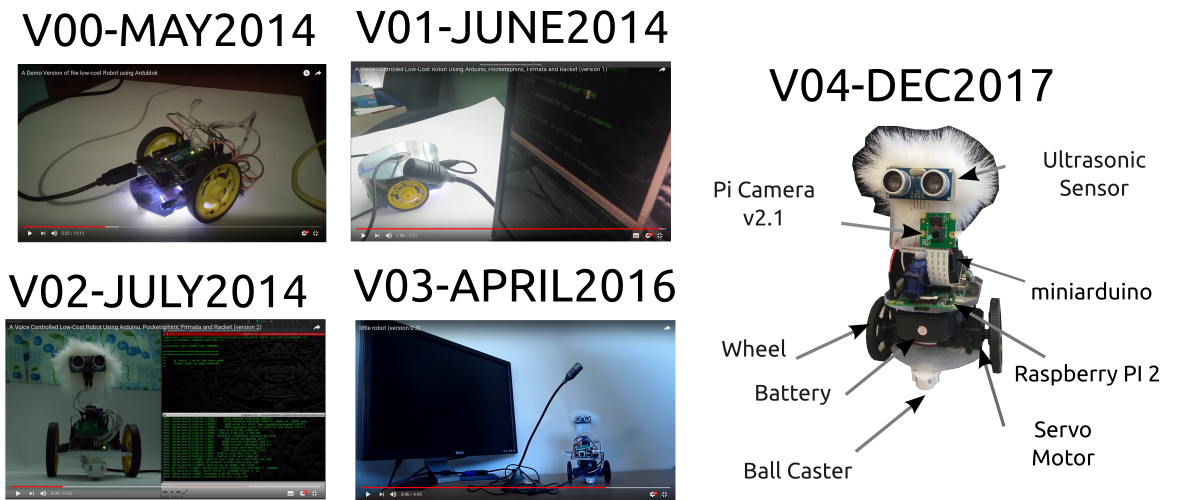
\includegraphics[width=1.0\textwidth]{./figures/air4children/versions/drawing-v00.png}
        %\caption{}
      \end{figure}
\end{frame}
}

%%%%%%%%%%%%%%%%%%%%%%%%%%%%%%%%%%%%%%%%%%%%%%%%%%%%%%%%
{
\paper{Xochicale M. 2015 in Mecate; Parra C. et al. 2016, \it{Otto DIY}}
\begin{frame}{Piloting robot prototypes}
      \begin{figure}
        \centering
        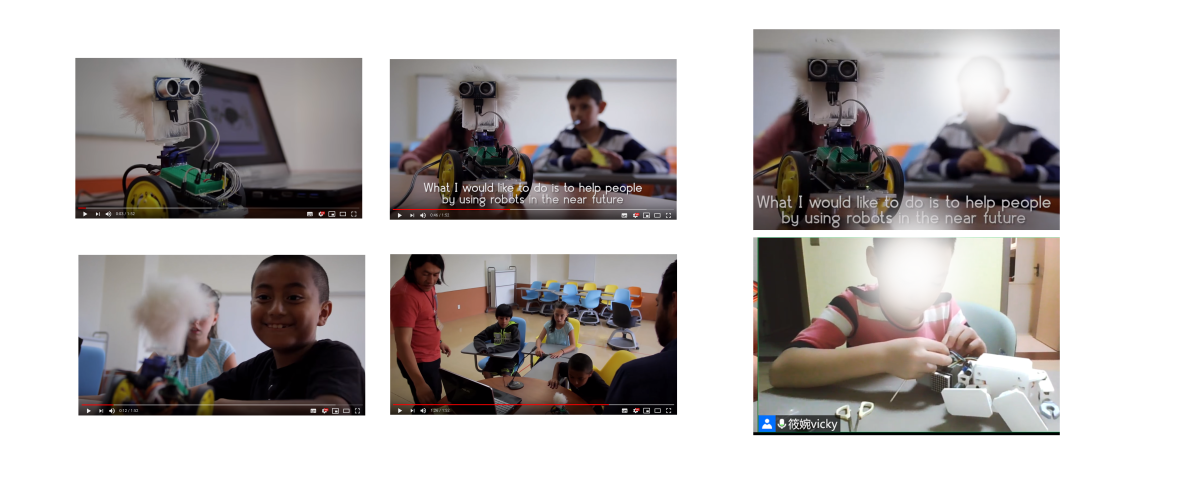
\includegraphics[width=1.0\textwidth]{./figures/air4children/versions/drawing-v01.png}
        %\caption{}
      \end{figure}
\end{frame}
}

%%%%%%%%%%%%%%%%%%%%%%%%%%%%%%%%%%%%%%%%%%%%%
\subsection{Teaching Materials based on Montessori Education and Spiral Learning}

%%%%%%%%%%%%%%%%%%%%%%%%%%%%%%%%%%%%%%%%%%%%%%%%%%%%%%%%
{
\paper{Elkin M., Sullivan A, Bers 2014 in Journal of Informantion and Technology}
\begin{frame}{Adopting Montessori Education in AIR4Children curriculum} 
  \vspace{3mm}
  \it{"The hand is the instrument of the mind."} Dr. Maria Montessori (1970-1952).
  \vspace{2mm}
    \begin{figure}
        \centering
        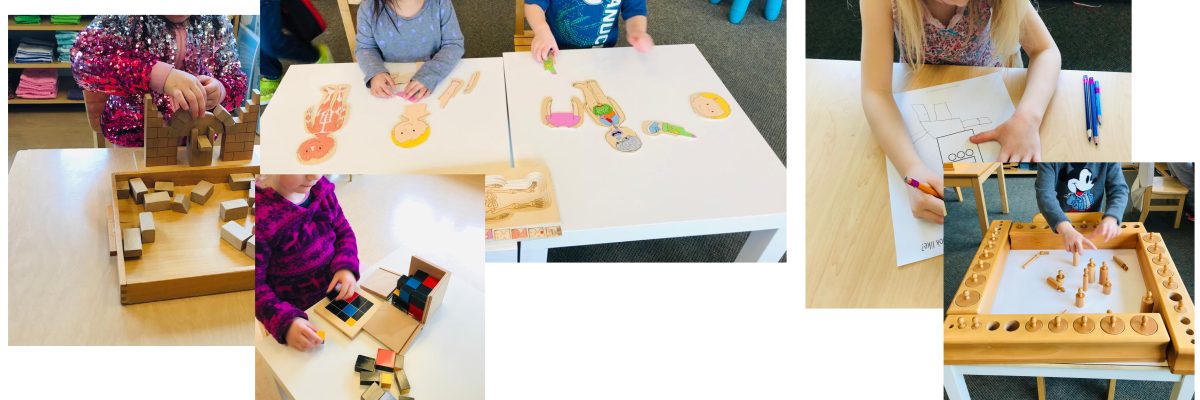
\includegraphics[width=1.0\textwidth]{./figures/montessori/versions/drawing-v00.png}
        %\caption{}
      \end{figure}
\end{frame}
}

%%%%%%%%%%%%%%%%%%%%%%%%%%%%%%%%%%%%%%%%%%%%%%%%%%%%%%%%
{
\paper{Mohammad T. et al., 2017; Harden R. M. 1999 in Journal of Medical Teacher}
\begin{frame}{Adopting Spiral Learning Methods in AIR4Children curriculum}

  \begin{figure}
        \centering
        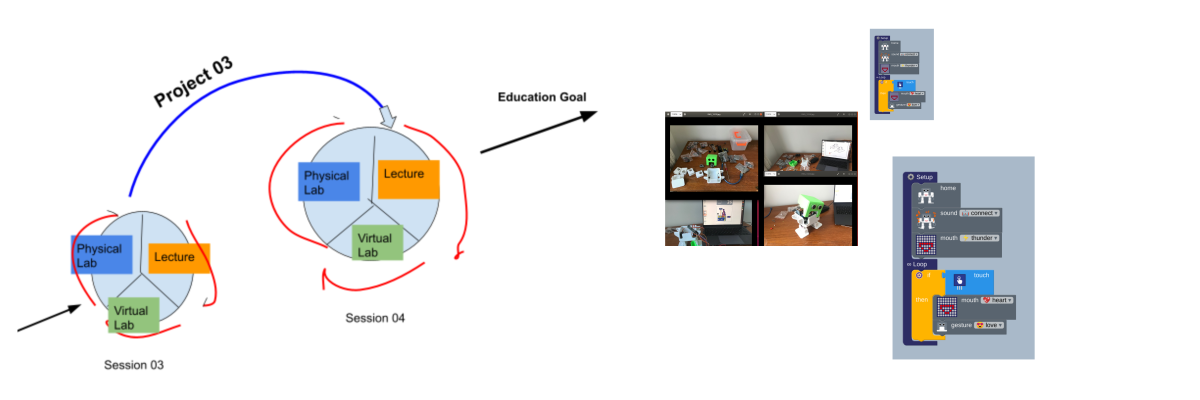
\includegraphics[width=1.0\textwidth]{./figures/teaching-materials/versions/drawing-v02.png}
        %\caption{}
      \end{figure}
\end{frame}
}

%%%%%%%%%%%%%%%%%%%%%%%%%%%%%%%%%%%%%%%%%%%%
\section{Conclusions and Future work}

%%%%%%%%%%%%%%%%%%%%%%%%%%%%%%%%%%%%%%%%%%%%%%%%%%%%%%%%
{
\paper{Lastname N. YEAR in journal of...}
\begin{frame}{Conclusions, future work and acknowledgements}

  \begin{columns}
    \begin{column}{.3\linewidth}
      Towards a more realistic
  \begin{itemize}
    \item \textbf{Fun}
    \item \textbf{Affortable}
    \item \textbf{Open Accessible}
    \item \textbf{D}
  \end{itemize}

    \end{column}


  \begin{column}{.6\linewidth}

      \begin{figure}
        \centering
        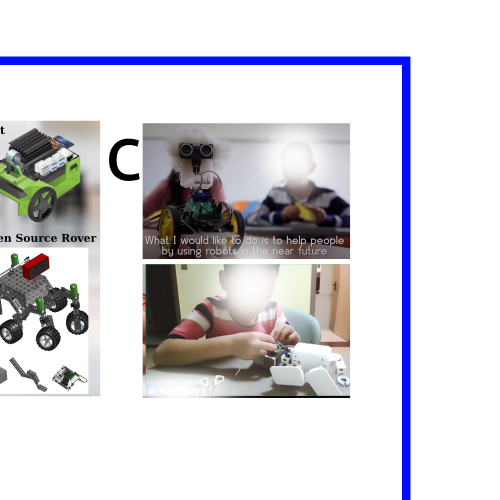
\includegraphics[width=0.9\textwidth]{./figures/future-work/versions/drawing-v00.png}
      \end{figure}

    \end{column}
  \end{columns}

\end{frame}
}


%%%%%%%%%%%%%%%%%%%%%%%%%%%%%%%%%%%%%%%%%%%%%%%%%%%%%%%%
{
\paper{Lastname N. YEAR in journal of...}
\begin{frame}{Acknowledgements}


      \begin{figure}
        \centering
        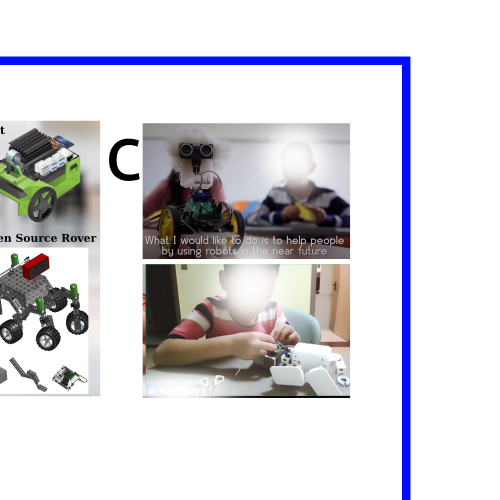
\includegraphics[width=0.9\textwidth]{./figures/future-work/versions/drawing-v00.png}
      \end{figure}


\end{frame}
}




%\begin{frame}[standout]
%  Thanks \\
%  Questions?
%\end{frame}

\maketitle

\end{document}
